%
% LaTeX2e template for FIT2010
%

%本テンプレートは *非公式* のものです.
%ご自身の責任においてご利用下さい.

\documentclass[a4j,twocolumn]{jarticle}
\usepackage[dvipdfmx]{graphicx}
\usepackage{amsmath,amssymb,amsfonts,amsthm,enumerate}
%\usepackage[dvips]{graphicx}


\makeatletter
% \sectionと\subsection部分のフォントサイズを10.5ポイントに設定します
% 参考URL http://www.h4.dion.ne.jp/~latexcat/intro/i7-r2.html
\def\section{\@startsection{section}{1}{\z@}%
   {0.6\Cvs}%
   {0.3\Cvs}%
   {\reset@font\fontsize{10.5pt}{0pt}\bfseries}}
\def\subsection{\@startsection{subsection}{2}{\z@}%
   {\Cdp}%
   {\Cdp}%
   {\reset@font\fontsize{10.5pt}{0pt}\bfseries}}
% 章番号の後にピリオドを入れます.
% 参考URL http://oku.edu.mie-u.ac.jp/~okumura/texfaq/qa/34044.html
\def\@seccntformat#1{\csname the#1\endcsname.}
\def\thefootnote{\fnsymbol{footnote}}
\makeatother


\def\baselinestretch{0.83}

% 各種マージンの設定
% 参考URL http://www.nsknet.or.jp/~tony/TeX/faq/layout.htm
\setlength{\oddsidemargin}{20mm}
\setlength{\evensidemargin}{20mm}
\addtolength{\oddsidemargin}{-1in}% デフォルトのマージンを引きます.
\addtolength{\evensidemargin}{-1in}% デフォルトのマージンを引きます.
\setlength{\textwidth}{170mm}% 210-20-20
\setlength{\topmargin}{30mm}
\addtolength{\topmargin}{-1in}% デフォルトのマージンを引きます.
\setlength{\headheight}{0mm}
\setlength{\headsep}{0mm}
\setlength{\textheight}{242mm}% 297-30(top)-25(bottom)
\setlength{\columnsep}{7mm}





% local settings
\usepackage{color}
\definecolor{purple}{rgb}{0.6,0,0.4}
\definecolor{brown}{cmyk}{0,0.81,1,0.60}
\definecolor{gray}{rgb}{0.4,0.4,0.4}
\definecolor{darkblue}{rgb}{0.0,0.0,0.6}
\definecolor{cyan}{rgb}{0.0,0.6,0.6}
\usepackage{listings,jlisting}
\renewcommand{\lstlistingname}{ソースコード}
\renewcommand{\slash}{/}
\lstdefinestyle{MyJava} % JavaとXML,2つの言語を使いたかったので.style=MyJavaとかで使い分け
{
language=Java, % lstlisting内の言語の指定
numbers=left, % 行番号を左端に表示する
breaklines = true, % 行が長くなってしまった場合の改行を行う
basicstyle={\small}, % 標準の書式設定
identifierstyle={\small}, % 識別子のスタイル
keywordstyle={\small\bfseries\color{purple}}, % キーワードのスタイル
commentstyle={\small\itshape\color{gray}}, % コメントのスタイル
stringstyle={\small\ttfamily\color{brown}}, % 文字列のスタイル
frame=single, % 枠のスタイル
tabsize=2, % タブ幅
showstringspaces=false, % 空白を可視化するか
}
\lstdefinelanguage{XML} % XMLはあまり充実してないってさー
{
    morestring=[b]",
    morestring=[s]{>}{<},
    morecomment=[s]{<?}{?>},
    stringstyle=\color{brown},
    identifierstyle=\color{darkblue},
    keywordstyle=\color{cyan},
    morekeywords={xmlns,version,type}% list your attributes here
}
\lstdefinestyle{MyXML} % JavaとXM(ry
{
language=XML,
numbers=left,
breaklines=true,
basicstyle={\small},
identifierstyle={\small\color{darkblue}},
keywordstyle={\small\bfseries\color{cyan}},
commentstyle={\small\itshape\color{gray}},
stringstyle={\small\ttfamily\color{brown}},
frame=single,
tabsize=2,
showstringspaces=false,
}
\usepackage{ascmac}
\usepackage{otf}
% end of local settings



\begin{document}
\pagestyle{empty}
\thispagestyle{empty}

\twocolumn[%
\begin{center}
 {\Large スマートフォンのモーションセンサを利用した個人認証アプリケーションの開発}\vspace{.5ex}

 {\Large\sffamily Development of Personal Authentication Application Using the Motion Sensor of a Smartphone}\vspace{1ex}


\large
\mbox{}
\hfil
\setcounter{footnote}{2}
{\bfseries \UTF{9AD9}坂賢佑}${}^\thefootnote$
\hfil
\setcounter{footnote}{2}
{\bfseries 平松耕輔}${}^\thefootnote$
\hfil
\setcounter{footnote}{3}
{\bfseries 小林孝史}${}^\thefootnote$
\hfil
\mbox{}

\mbox{}
\hfil
{\sffamily Kensuke Kosaka}
\hfil
{\sffamily Kosuke Hiramatsu}
\hfil
{\sffamily Takashi Kobayashi}
\hfil
\mbox{}
\hfil

\end{center}
]

\setcounter{footnote}{2}
\footnotetext{関西大学大学院総合情報学研究科}
\setcounter{footnote}{3}
\footnotetext{関西大学総合情報学部}

\section{はじめに}
スマートフォンが普及しつつある現在,スマートフォンにおける個人認証の方法は画面上に表示されるソフトウェアキーボードのテンキーパッドを用いたパスコード認証と指紋認証が大部分を占めている.
しかし,パスコード認証を用いる場合は画面ロックを解除するたびに画面に表示されたソフトウェアキーボードを目で見て指でタッチして操作する必要があり,ユーザにとって煩雑な作業である.
また,パスコードはあらかじめ決められた文字種の中から一つずつ文字を選択し,これを並べて構築していく.
この性質上パスコードのパターン数は限られてしまい,認証に用いる鍵の自由度が制限されてしまう.

指紋認証を用いる場合は,認証を行う際に指紋の読み取りモジュールに指を重ねるだけなのでユーザにかかる負担は比較的軽い.
だが,指紋認証を行うためには指紋を読み取るための専用のハードウェアが必要である.
また,指紋そのものは変更できない.
そのため指紋情報が万が一第三者に漏洩した可能性がある場合,今後はその指を認証に用いることができなくなるという問題点がある.

そこで,本研究では人間の動き(以下,モーション)を用いた個人認証アプリケーションを開発する.
これによりパスコード認証が抱える認証の煩雑さを軽減し,かつ認証に用いる鍵の情報が漏洩した際にも鍵の変更が可能となる.
加えて,モーションを鍵とすることで,自由度が高くより直感的に個人認証が行える.
このアプリケーションには,一般的なスマートフォンに搭載されている加速度センサと角速度センサを用いる.


\section{関連研究}
坂本の研究\cite{sakamoto}では,ユーザが入力したモーションの数値化に加速度センサを用いた.
あらかじめ保存しておいた複数種類のジェスチャパターンと認証時にユーザが入力したモーションデータをパターンマッチング方式のアルゴリズムを用いて比較することで個人認証を行った.
しかし,このプログラムは扱うジェスチャによって認証率が高いものと低いものに二分化する傾向が見られるという問題点があった.

\UTF{6FF5}野らの研究\cite{hamano}では,加速度センサに加えて角速度センサを用いたジェスチャ動作による認証手法を提案した.
これにより回転動作の取得によるモーションの自由度向上となりすまし認証に対する強度の向上を可能にした.
認証手法として単一動作を組み合わせて認証する単一動作組み合わせ認証と,ユーザが自由に考えたモーションを用いてDPマッチングによって認証する一筆書き認証の二つを提案した.
%単一動作組み合わせ認証では,モーション入力より得られた加速度データ・角速度データのそれぞれx,y,z軸の六つのラベルからもっとも分散の大きいものをジェスチャパターンとして識別する.
%識別したジェスチャパターンをパスワードのように組み合わせ,登録されたジェスチャパターン列と一致しているかを判定することで認証した.
%一筆書き認証では,あらかじめ登録されたマスタデータと新たに入力したサンプリングデータをDPマッチングを用いて類似度を比較し,あらかじめ定められた閾値を用いて認証した.
%この研究ではモーションデータに含まれる手振れなどの微小なノイズを除去するために移動平均を施しており,モーション入力毎の時間や速度の差異を抑えるためにデータ長や振幅の正規化を行っている.
%実験より,初日の本人拒否率の平均が一筆書き認証では61\%,単一動作組み合わせ認証では52\%となった.
%また筆者自身がなりすました際の他人受容率の平均が一筆書き認証では12\%,単一動作組み合わせ認証では24\%となった.
このシステムの実証実験は複数日かけて実施されており,一筆書き認証において日を経ることによる習熟度の向上から,本人拒否率が改善したことが確認された.
しかし,初日の認証での本人拒否率が高く,さらなる本人拒否率の改善が課題として挙げられていた.


% @suppress InvalidSymbol
\section{本研究のシステム}
本研究では兎澤の研究で挙げられていた全体的な認証成功率の低さ,特に手首を中心とする比較的動きの小さいモーションでの認証成功率の改善を目標とする.
また,特定の図形や記号を元にしたモーションだけでなく,端末を上下に振るなどより単純で日常的な入力が容易なモーションであっても利用が可能なシステムの実装を目指す.
システムの動作フローを図\ref{flow}に示す.

\begin{figure}[bthp]
    \centering
    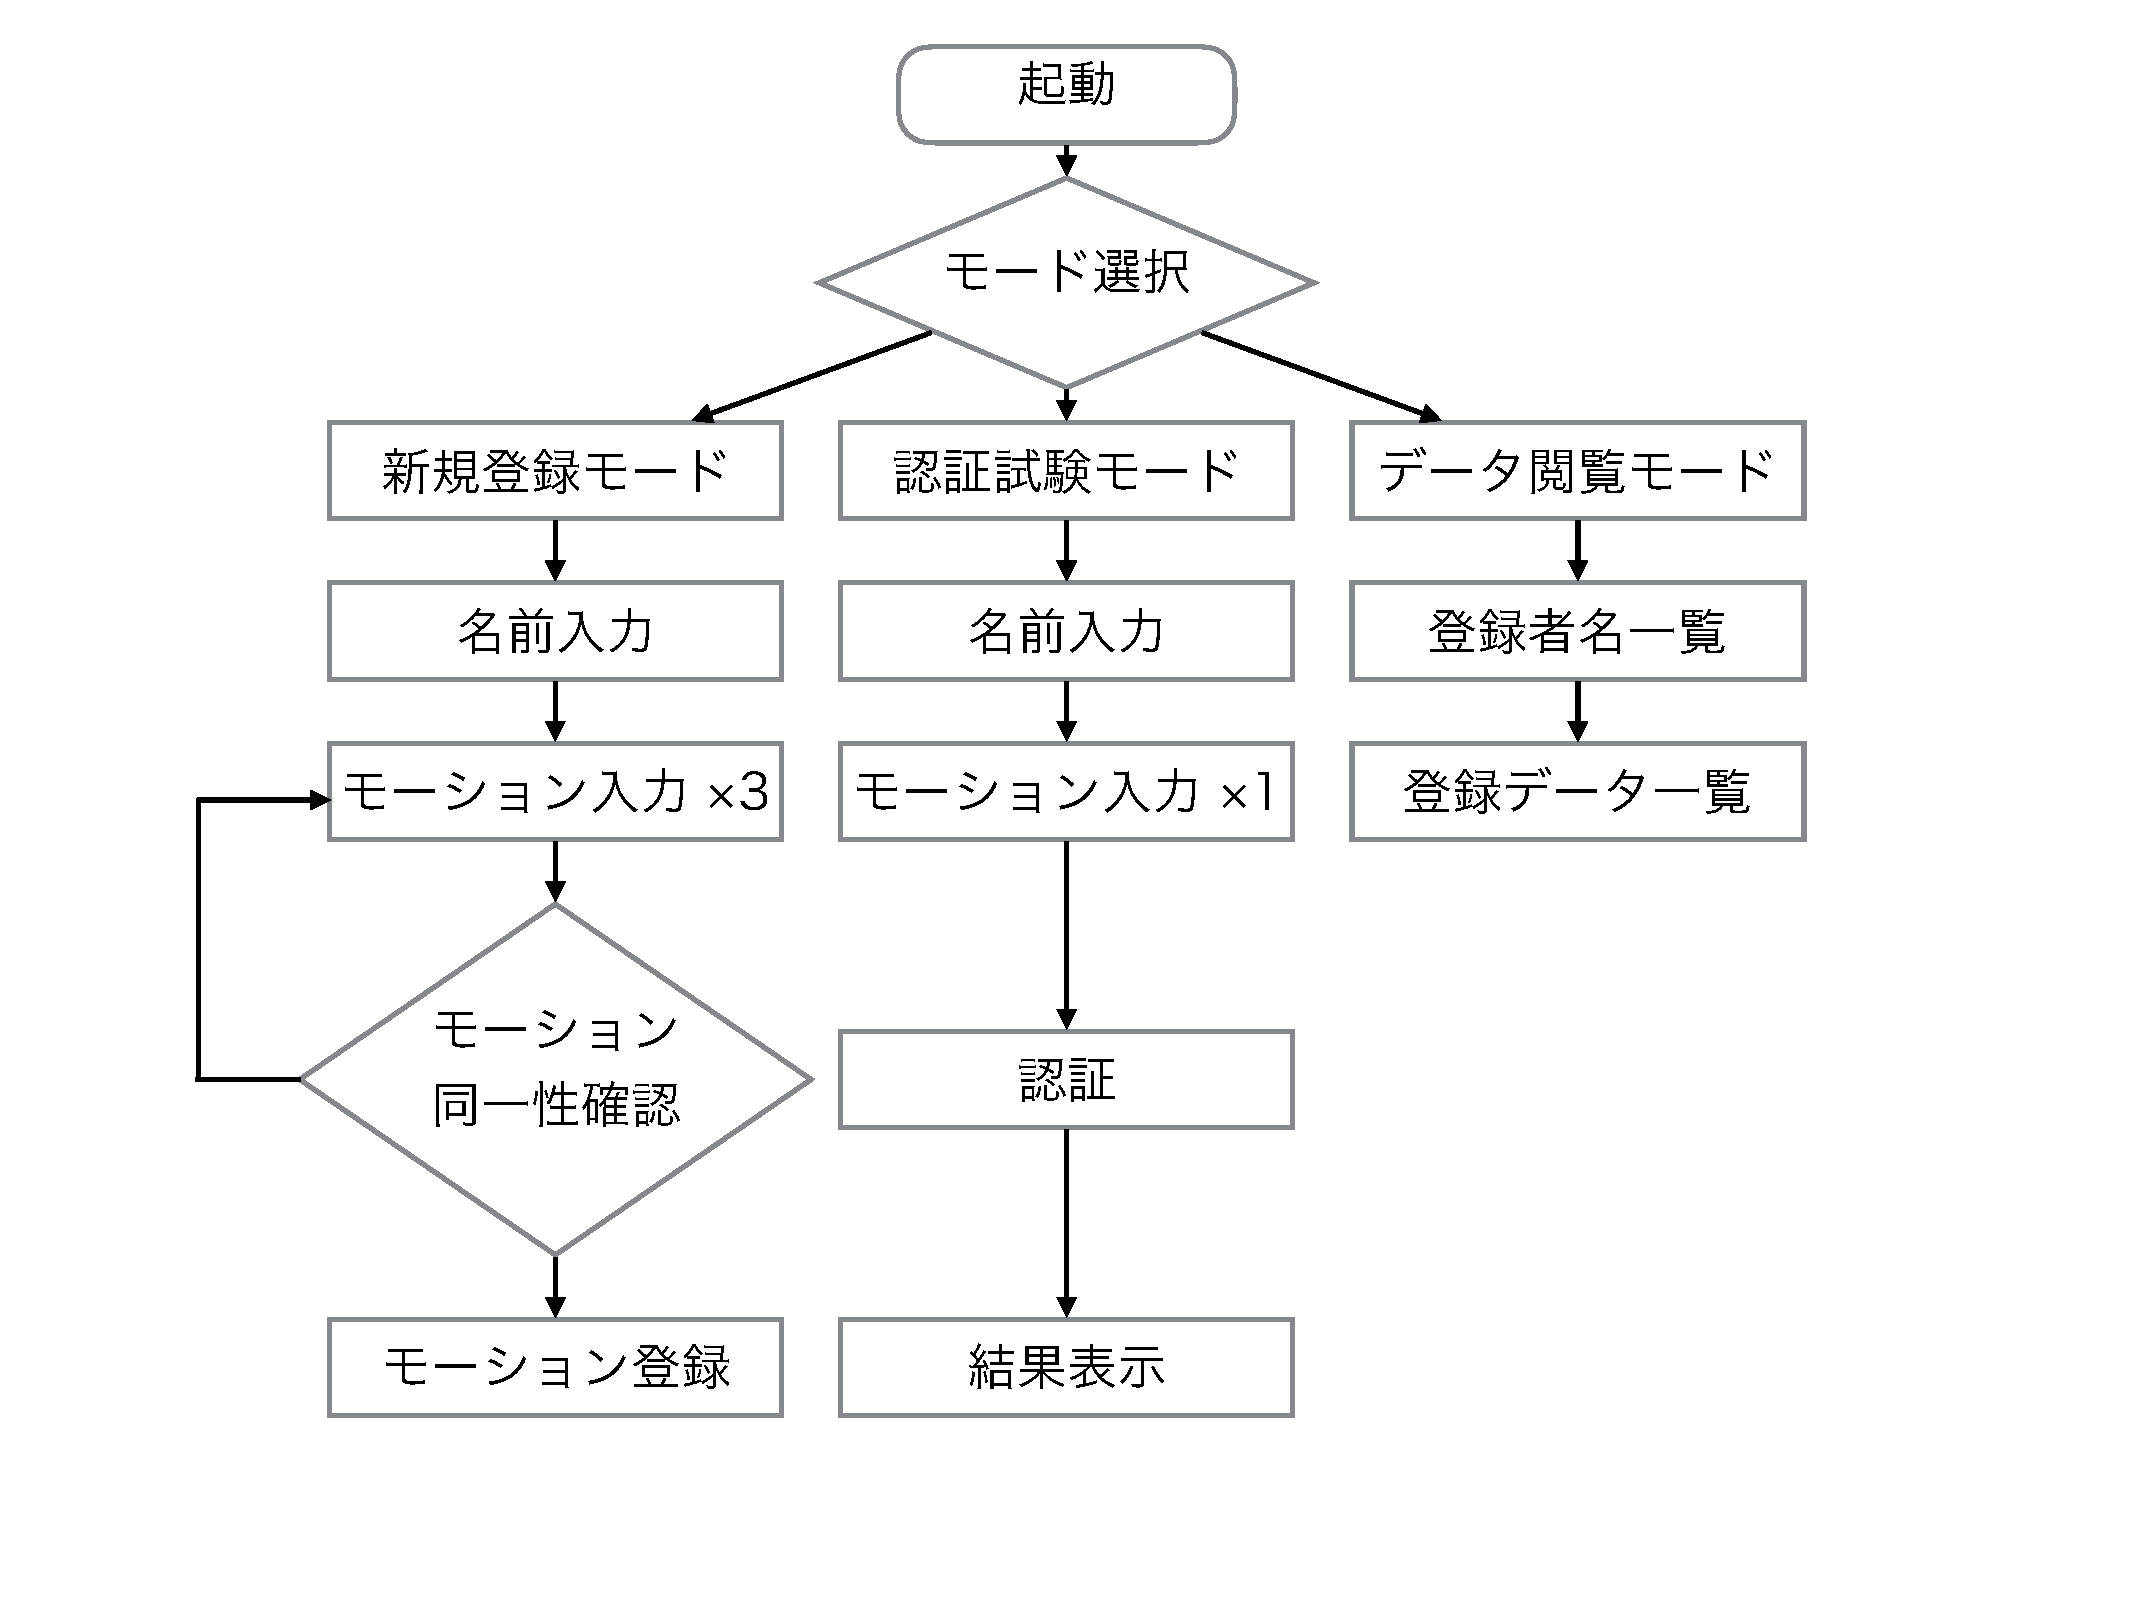
\includegraphics[bb=0 100 950 750, width=80mm]{flow.pdf}
    \caption{アプリケーション動作フロー}
    \label{flow}
\end{figure}

アプリケーション起動時に表示されるモード選択ダイアログから,ユーザはまず新規登録モードを選択する.
このモードでは,ユーザ名を指定して個人認証を行う際の鍵情報となるモーションを登録できる.
モード選択後登録したいユーザ名を入力し,モーションの入力を任意の長さで3回行う.
データを取得した後に最も入力時間の長かったデータを基準に他のデータの末尾にゼロを補填する方法でデータの長さを揃え,その後データの振れ幅を確認する.
あらかじめ設定しておいた増幅器の閾値を元に,取得したデータの振れ幅が下回った場合はモーションの動きが小さいとし,全てのデータに増幅量を掛けることで振れ幅の増幅処理を行う.
次にフーリエ変換を用いたローパスフィルタ処理によって,モーション入力時の手の震えなどから生じうるデータへの影響を取り除く.
ローパスフィルタ処理が終われば加速度データから距離を,角速度データから角度を求め,コサイン類似度を用いて取得したデータが同一のモーションであるかの確認を行う.
同一のモーションであればモーション入力時に生じうる時間的なズレを修正する.
同一のモーションでなければモーションの取り直しを行う.
時間的なズレを修正する処理が終われば処理を行った3回分のデータから平均値を求め,これを増幅量とともに登録する.
登録する際は暗号化方式に鍵長128ビットのAESを,パディング方式にPKCS\#5 Paddingを,暗号利用モードにCBCを用いた暗号化処理をデータに施したものを端末に保存する.

これらの処理を行うことで,兎澤の研究であげられていた認証成功率の低さや対応できるモーションに限りがあるという問題に対処している.

認証試験モードでは,あらかじめ新規登録モードにおいてモーションの登録を行ったユーザ名を指定する.
指定されたユーザ名で既にモーションの登録がなされていることが確認できた場合のみ,モーションの入力画面に移る.
認証試験モードでは,モーションの入力を任意の長さで1回行う.
データを取得した後に,登録されたデータの長さを基準にデータの長さが短い場合は末尾にゼロを補填し,長い場合は末尾を切り落とす方法で揃える.
その後新規登録モードにおいてモーションデータとともに登録された増幅量を元に,取得したデータに対して増幅処理を行う.
そしてフーリエ変換を用いたローパスフィルタ処理を行い,加速度データから距離を,角速度データから角度を求める.
これらの処理によって得られたデータと登録されたデータとのコサイン類似度を求め,個人認証を行う.

データ閲覧モードでは,新規登録モードにおいて登録されたユーザ名及びモーションデータを,リスト形式で閲覧できる.


% @suppress
\section{評価及び考察}
本システムの有用性を確認するため,実験を行った.
13名の被験者に協力してもらい,円・三角・寝かせて起こす・顔に近づける・上下に2往復振る,という五つのモーションについてそれぞれ入力してもらった.
登録及び認証の試行回数は3回までとし,この回数内で登録及び認証できた場合に成功とした.
被験者には各モーションのそれぞれについて,まず登録をしてもらい,登録できた場合はすぐに認証をしてもらった.
この実験より得られた結果について,モーション及びユーザ毎の登録及び認証の成功率をまとめたものを表\ref{test}に示す.

\begin{table}[htbp]
    \centering
    \caption{モーション及びユーザ毎の登録及び認証の成功率}
    \begin{tabular}{c}
        \begin{minipage}{0.46\hsize}
            \centering
            \begin{tabular}{|c|r|r|} \hline
                & 登録 & 認証 \\ \hline
                circle & 92\% & 91\% \\ \hline
                triangle & 92\%  & 75\% \\ \hline
                lay & 53\% & 100\% \\ \hline
                face & 53\% & 100\% \\ \hline
                shake & 76\% & 90\% \\ \hline
            \end{tabular}
        \end{minipage}
        \begin{minipage}{0.46\hsize}
            \centering
            \begin{tabular}{|c|r|r|} \hline
                & 登録 & 認証 \\ \hline
                A & 80\% & 100\% \\ \hline
                B & 80\% & 75\% \\ \hline
                C & 100\% & 100\% \\ \hline
                D & 60\% & 66\% \\ \hline
                E & 60\% & 100\% \\ \hline
                F & 100\% & 80\% \\ \hline
                G & 40\% & 100\% \\ \hline
                H & 100\% & 80\% \\ \hline
                I & 60\% & 66\% \\ \hline
                J & 40\% & 100\% \\ \hline
                K & 60\% & 100\% \\ \hline
                L & 100\% & 100\% \\ \hline
                M & 80\% & 100\% \\ \hline
            \end{tabular}
        \end{minipage}
    \end{tabular}
    \label{test}
\end{table}

また,この実験を行うにあたり,登録と認証において被験者がモーションを入力する様子を肩越しに見るような角度でビデオ撮影した.
全てのモーションについて登録及び認証が成功した被験者Cと被験者Lを対象に,この撮影データを用いて3回までの試行でなりすまし認証が可能か確認した.
得られた結果について,各被験者の各モーション毎に3回の試行で最も高かったコサイン類似度をまとめたものを表\ref{spoof}に示す.

\begin{table}[htbp]
    \centering
    \caption{なりすまし認証でのコサイン類似度}
    \begin{tabular}{|c|r|r|r|r|} \hline
        & \multicolumn{2}{|c|}{C} & \multicolumn{2}{|c|}{L} \\
        & 距離 & 角度 & 距離 & 角度 \\ \hline
        circle & 0.21 & 0.04 & 0.08 & -0.24 \\ \hline
        triangle & 0.11 & -0.19 & -0.12 & -0.13 \\ \hline
        lay & -0.06 & -0.27 & -0.16 & 0.02 \\ \hline
        face & 0.34 & 0.50 & 0.45 & 0.55 \\ \hline
        shake & 0.28 & 0.09 & 0.03 & 0.20 \\ \hline
    \end{tabular}
    \label{spoof}
\end{table}

表\ref{test}から,端末を寝かせて起こすモーションや顔に近づけるモーション,端末を上下に振るモーションといった単純なモーションについて認証が可能であることがわかった.
しかし,全てのモーションについて登録及び認証が成功した被験者が2名しかおらず,成功しやすい被験者と失敗しやすい被験者に二分化する傾向が見られた.
また,被験者から登録や認証に成功するために馴れが必要であるとの声が聞かれた.

表\ref{spoof}から,ほぼ全てのなりすまし認証は失敗したが,被験者Lの顔に近づけるモーションでのなりすまし認証のみ成功する結果となった.
現在のシステムでは,認証の可否を判断する際に距離と角度のコサイン類似度の平均が0.5を上回った場合に認証成功としている.
今回なりすまし認証が成功したケースでは距離についてコサイン類似度が0.45であるにもかかわらず,角度のコサイン類似度が0.55であるために平均すると0.5を越える結果となった.
角度のコサイン類似度が高くても距離のコサイン類似度が低ければ同一のモーションとは考えにくい.
距離と角度それぞれについてコサイン類似度が閾値を越えているかを判断し,これによって認証の可否を判断するように改善する必要がある.



\bibliographystyle{plain}
\begin{thebibliography}{9}
    \bibitem{sakamoto}坂本翔,ユーザの直感的な入力をとらえるための3軸加速度センサによるジェスチャ認識の研究,2009年度公立はこだて未来大学卒業論文.
    \bibitem{tozawa}兎澤星伸,三軸加速度センサ及び三軸ジャイロセンサを用いた認証アプリケーションの開発,2012年度関西大学卒業研究.
\end{thebibliography}


\end{document}
